\newpage
\section{Diagramas de secuencia}
A continuación se describe la interacción de nuestras entidades de negocio y el ciclo de vida que tendrán en la aplicación. También se detalla la interacción, mensajes y la lógica implementada en cada uno de los diferentes escenarios.\par

\subsection{DS1. Inicio de sesión}
El inicio de sesión consiste en la captura de usuario y contraseña de una cuenta para tener acceso a sus datos. Estos dos datos se envían en formato JSON a AWS API Gateway que sirve de puerta de enlace para poder establecer una comunicación con la AWS Lambda \textit{ARFLogin} la cual se encarga de realizar una consulta en una base de datos en MySQL montada sobre una instancia de AWS RDS para verificar que los datos correspondan a una cuenta registrada. El resultado de esta consulta, ya sea exitosa o fallida, se devuelve a ARF en formato JSON a través de AWS API Gateway. Esta respuesta tiene dos parámetros que indican el estatus de la operación: \textbf{code} y \textbf{message}

\begin{figure}[h!]
	\centering
	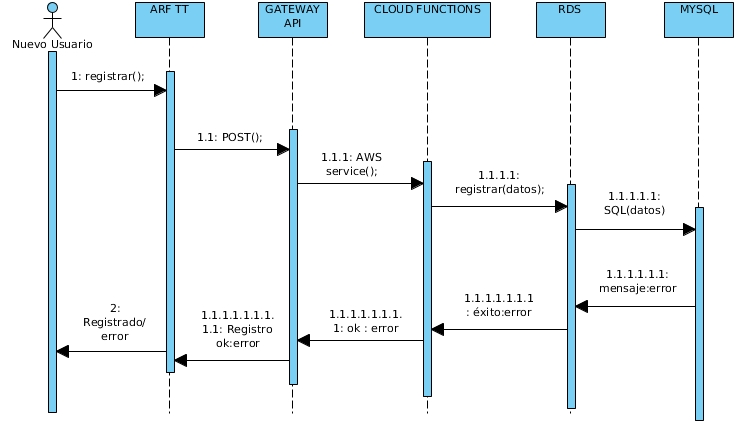
\includegraphics[width=14cm,height=8cm]{imagenes/analisis/DSregistrarUsuario.jpg}
	\caption{DS1. Inicio de sesión.}
	\label{fig:dsiniciosesion}
\end{figure}